\chapter{Analýza sentimentu}\label{sentiment}

V předchozí kapitole~\ref{kapitola1} bylo ukázáno, jak počítače zpracovávají lidský jazyk, a také byly představeny moderní jazykové modely založené na transformátorové architektuře. Tato kapitola bude zamířena na jedno z důležitých využití NLP a jazykových modelů -- \emph{analýzu sentimentu}, jež představuje hlavní téma této práce.

S rozvojem internetu získali lidé z nejrůznějších prostředí prostor pro veřejné komentáře a sdílení názorů -- ať už jde o recenze produktů, diskuze o politice nebo komentáře ke známým osobnostem. Každý den tak vzniká obrovské množství textových dat, která sama o sobě nenabízejí přímou hodnotu. Již kolem roku 2003 proto začaly vznikat první výzkumy~\cite{NasukawaSA}, jejichž cílem bylo najít způsoby, jak tuto textovou \uv{zpětnou vazbu} analyzovat a využívat v praxi. Firmy tak mohou pomocí analýzy sentimentu odhalit postoje svých zákazníků, lépe řídit vývoj nových produktů a cíleněji směřovat své služby.~\cite{Aqlanstudyofsentiment}

Analýza sentimentu, někdy nazývaná také \emph{opinion mining}, slouží k zjišťování názorů, pocitů a reakcí uživatelů na internetu, zejména na sociálních sítích či obchodních portálech. Typicky se využívá ke klasifikaci textů (např. recenzí či komentářů) do kategorií \uv{pozitivní}, \uv{negativní} a \uv{neutrální}. S rozmachem sociálních sítí se oblasti, které chtějí pochopit názory uživatelů -- jako politici, výrobci, vědci či psychologové --, zaměřují právě na tuto formu textové analýzy. Analýza sentimentu stojí na kombinaci metod zpracování přirozeného jazyka (NLP), statistiky a strojového učení, a snaží se tak efektivně zachytit a definovat \uv{náladu} či postoj v textu.~\cite{Aqlanstudyofsentiment}

Analýza sentimentu se nemusí omezovat pouze na psaný text, protože emoce a postoje lze rozpoznávat i z dalších druhů obsahu. Například v řečovém projevu se vyhodnocuje tón hlasu, rytmus, intonace a způsoby vyjadřování, z nichž lze usuzovat zaujetí či emocionalitu mluvčího. U fotografií nebo videí se pak zkoumají neverbální signály, jako jsou mimika, gesta a celková kompozice, které mohou vypovídat o náladě či názoru zobrazovaných osob. Dalším příkladem jsou tzv. memy, podle kterých se dá sledovat nálada uživatele, který tento meme zveřejnil. Pokud se propojí více druhů médií (audio, video a text), hovoříme o tzv. \emph{multimodální analýze sentimentu}.~\cite{kumar2023comprehensivereviewsentimentanalysis} V této práci se však pozornost soustředí výhradně na analýzu sentimentu v textu.

\section{Techniky analýzy sentimentu}\label{TechAnaSen}
K analýze sentimentu lze přistupovat různými způsoby, které se liší technickým zázemím i mírou využití jazykových modelů, představených v sekci~\ref{LM}. Zpravidla se rozlišují metody slovníkové (lexicon-based), tradiční přístupy strojového učení, hluboké učení (neuronové sítě) a hybridní řešení. K modernějším technikám pak patří postupy založené na transformátorové architektuře (viz podsekce~\ref{Transformator}). Podrobný přehled výhod a nevýhod těchto metod i jejich konkrétních možností nasazení lze nalézt v díle~\cite{MAO2024102048}.

V této práci je pro analýzu sentimentu zvolen přístup využívající transformátorové modely, jak bylo podrobněji popsáno v sekci~\ref{PLMs}. Díky mechanismu pozornosti (attention) tyto modely lépe zachycují kontext a jemné jazykové nuance, a proto mnohdy překonávají klasické techniky analýzy sentimentu v přesnosti i rozsahu využití.

\subsection{Slovníková metoda}
Slovníkový přístup vychází z předpokladu, že některá slova bývají tradičně vnímána jako \uv{pozitivní} a jiná jako \uv{negativní}. Tato slova se shromažďují v tzv. slovnících (lexikonech), podle nichž se následně určuje sentiment textu. Rozlišují se přitom dva základní postupy, korpusový a slovníkový, přičemž každý z nich má své specifické výhody i nevýhody. Detailnější přehled této metody lze nalézt v pracích~\cite{Aqlanstudyofsentiment, MAO2024102048}.

\subsection{Tradiční přístupy strojového učení}
Tradiční metody strojového učení vycházejí z rozdělení dat na trénovací a testovací sadu. Model se na trénovací sadě naučí rozlišovat sentiment (případně jiné charakteristiky) a poté se ověří na dosud neviděných datech z testovací sady. Příkladem takových postupů jsou Naivní Bayes (NB), Metoda podpůrných vektorů (SVM) nebo rozhodovací stromy~\cite{MAO2024102048}. Různé studie zkoumající nasazení těchto tradičních metod v analýze sentimentu jsou přehledně popsány v~\cite{SuryawanshiSA}.

\subsection{Hluboké učení}
Kvůli nedostatečnému výpočetnímu výkonu nebylo možné hluboké učení (neuronové sítě) důkladně zkoumat. Avšak díky výraznému technologickému pokroku, zejména v oblasti grafických procesorů (GPU), získaly neuronové sítě na výkonnosti a možnosti využití. Hluboké učení využívá kaskádu více vrstev nelineárních zpracovatelských jednotek pro extrakci a transformaci příznaků. Nižší vrstvy, které jsou blízko vstupním datům, se učí jednoduché rysy, zatímco vyšší vrstvy zachycují složitější vlastnosti, jež jsou odvozeny z příznaků získaných v nižších vrstvách.~\cite{zhang2018deeplearningsentimentanalysis}

V této sekci budou představeny nejpoužívanější typy neuronových sítí v oblasti NLP, a to zejména konvoluční neuronové sítě (\emph{Convolutional Neural Networks, CNN}), rekurentní neuronové sítě (\emph{Recurrent Neural Networks, RNN}) a sítě s dlouhou krátkodobou pamětí (\emph{Long Short Term Memory networks, LSTM}). Jednotlivé typy neuronových sítí jsou zde popsány pouze stručně, zatímco podrobnější informace lze nalézt v díle~\cite{zhang2018deeplearningsentimentanalysis}. Přehled studií zkoumajících využití těchto metod v praxi je uveden v~\cite{SuryawanshiSA}.

\subsubsection{Konvoluční neuronové sítě}
Konvoluční neuronová síť (CNN) je druh dopředné neuronové sítě, který byl původně vyvíjen pro úlohy spojené s počítačovým viděním. Její architektura čerpá inspiraci z lidské zrakové kůry (vizuální mechanismus přítomný v mozku živočichů). Tato zraková kůra obsahuje početné skupiny buněk citlivých na světlo v malých, vzájemně se překrývajících oblastech zorného pole, jež se označují jako receptivní pole. Tyto buňky fungují jako lokální filtry, které přenášejí informace o vstupních signálech dále. CNN se proto skládá z několika konvolučních vrstev, přičemž každá vrstva napodobuje funkci zmíněných buněk v zrakovém centru.~\cite{zhang2018deeplearningsentimentanalysis}

\subsubsection{Rekurentní neuronové sítě}
Rekurentní neuronová síť (RNN)~\cite{RNNbib} je typ neuronové sítě, ve které jsou spojení mezi neurony uspořádána do směrovaného cyklu. Na rozdíl od dopředných neuronových sítí dokáže díky své vnitřní  \uv{paměti} zpracovávat i sekvenční data. Tato  \uv{paměť} znamená, že pro každý prvek vstupní sekvence používá RNN stejné operace, přičemž výstup v každém kroku závisí na všech dosavadních výpočtech. Tímto způsobem si RNN  \uv{pamatuje} kontext již zpracovaných prvků a uplatňuje jej při dalším výpočtu.~\cite{zhang2018deeplearningsentimentanalysis}

\subsubsection{Sítě s dlouhou krátkodobou pamětí}
Síť s dlouhou krátkodobou pamětí (LSTM)~\cite{LSTMbib} představuje speciální druh RNN schopný pracovat s dlouhodobými závislostmi. Všechny RNN lze popsat jako řetězec opakujících se modulů, avšak u klasické RNN je tento modul zpravidla jednoduchý, zatímco LSTM využívá složitější vnitřní strukturu. Namísto jedné vrstvy neuronů obsahuje čtyři, které spolu vzájemně specifickým způsobem komunikují.~\cite{zhang2018deeplearningsentimentanalysis}

\subsubsection{Další metody hlubokého učení v NLP}
Neuronové sítě a hluboké učení nejsou omezeny pouze na výše popsané tři typy. Existuje řada dalších přístupů a využití, která zde budou zmíněna jen stručně, podrobnější informace lze nalézt v díle~\cite{zhang2018deeplearningsentimentanalysis}.

\paragraph{Mechanismus pozornosti s RNN}
Aby bylo možné lépe zachytit dlouhodobé závislosti, s nimiž měly RNN a LSTM obtíže, začal se využívat mechanismus pozornosti, inspirovaný vizuální pozorností u člověka. Prvně byl aplikován u strojového překladu v NLP~\cite{bahdanau2016neuralmachinetranslationjointly}. Tyto sítě využívaly strukturu \emph{encoder-decoder}, která byla již letmo představena v sekci~\ref{DECENC} a později se stala hlavním stavebním kamenem transformátorové architektury.~\cite{zhang2018deeplearningsentimentanalysis}

\paragraph{Paměťové sítě}
Paměťové sítě (\emph{Memory networks, MemNN}) byly původně představeny v souvislosti s úlohou odpovídání na otázky~\cite{weston2015memorynetworks}. Využívají několik inferenčních komponent v kombinaci s velkou dlouhodobou pamětí, přičemž tyto komponenty mohou být tvořeny neuronovými sítěmi. Na jejich základě vznikla vylepšená verze End-to-End paměťová síť (\emph{End-to-End Memory network, MemN2N})~\cite{sukhbaatar2015endtoendmemorynetworks}, která kombinuje mechanismus pozornosti a práci s dlouhodobou pamětí.~\cite{zhang2018deeplearningsentimentanalysis}

\paragraph{Rekurzivní neuronové sítě}
Rekurzivní neuronové sítě (\emph{Recursive neural networks, RecNN}) představují typ neuronových sítí, které se obvykle používají k práci s řízenými acyklickými grafy (typicky stromovými strukturami). Jedná se o obecnější variantu rekurentních neuronových sítí (RNN).~\cite{zhang2018deeplearningsentimentanalysis}


\subsection{Hybridní metoda}
Jak název napovídá, hybridní metoda propojuje více přístupů -- například kombinuje charakteristiky slovníkových metod a strojového učení, aby využila silné stránky jednotlivých modelů a kompenzovala jejich slabiny~\cite{Aqlanstudyofsentiment}.

\section{Úrovně analýzy sentimentu}

Výzkumníci obvykle zkoumají sentiment na třech základních úrovních podrobnosti: \emph{dokumentové}, \emph{větné} a \emph{aspektové}.~\cite{MAO2024102048, zhang2018deeplearningsentimentanalysis}

\subsection{Dokumentová úroveň}
Klasifikace na dokumentové úrovni posuzuje celý text (např. recenzi produktu) jako jeden celek a určuje, jaký vyjadřuje postoj. Dokument se typicky zaměřuje na jednu entitu (např. \uv{telefon}) a snaží se posoudit její celkový sentiment.~\cite{zhang2018deeplearningsentimentanalysis}

Z pohledu analýzy sentimentu se v rámci této úrovně často pracuje jako s klasifikací dokumentu do tří tříd (pozitivní, negativní a neutrální). Tradičně se využíval přístup \emph{Bag of Words}, který s textem zachází jako s množinou slov bez ohledu na pořadí. O výsledném sentimentu rozhodovala frekvence nebo přítomnost určitých výrazů. Později se začaly prosazovat neuronové sítě, které využívají kódování slov do tzv. \emph{dense vectors}, které dokáží zakódovat informace o sémantických a syntaktických vlastnostech. Podrobnější informace o těchto přístupech a přehled výzkumů zaměřených na dokumentovou úroveň sentimentu lze nalézt v~\cite{zhang2018deeplearningsentimentanalysis}.

\subsection{Větná úroveň}
Na této úrovni se sentiment klasifikuje pro jednotlivé věty v textu. Obvykle se nejprve rozhoduje, zda věta vůbec vyjadřuje názor či nikoliv (tzv. \emph{subjectivity classification}), a teprve následně se stanovuje, jestli je vyjádřený sentiment pozitivní, negativní, nebo neutrální (tzv. \emph{polarity classification})~\cite{zhang2018deeplearningsentimentanalysis}.

Samotná predikce sentimentu pak probíhá podobně jako u dokumentové úrovně, ale vzhledem ke kratšímu rozsahu vět lze efektivněji využít i detailnější syntaktické a sémantické informace. Podrobnější informace o analýze sentimentu na větné úrovni a přehled souvisejících výzkumů jsou uvedeny v~\cite{zhang2018deeplearningsentimentanalysis}.

\subsection{Aspektová úroveň}
Aspektová úroveň představuje nejdetailnější formu analýzy sentimentu, protože nezkoumá pouze celkový sentiment textu, ale soustředí se na jednotlivé vlastnosti (\emph{aspekty} nebo \emph{cíle}) konkrétní entity.~\cite{zhang2018deeplearningsentimentanalysis} Tato úroveň představuje hlavní zaměření této práce, neboť umožňuje nejpřesněji interpretovat recenze či analyzovat mediální texty, například s cílem zjistit, jak jsou v novinových článcích hodnoceny různé firmy nebo osobnosti. Podrobnější popis celé problematiky aspektové analýzy sentimentu bude v následující sekci~\ref{absa}.

\begin{figure}[!htbp]
    \centering
    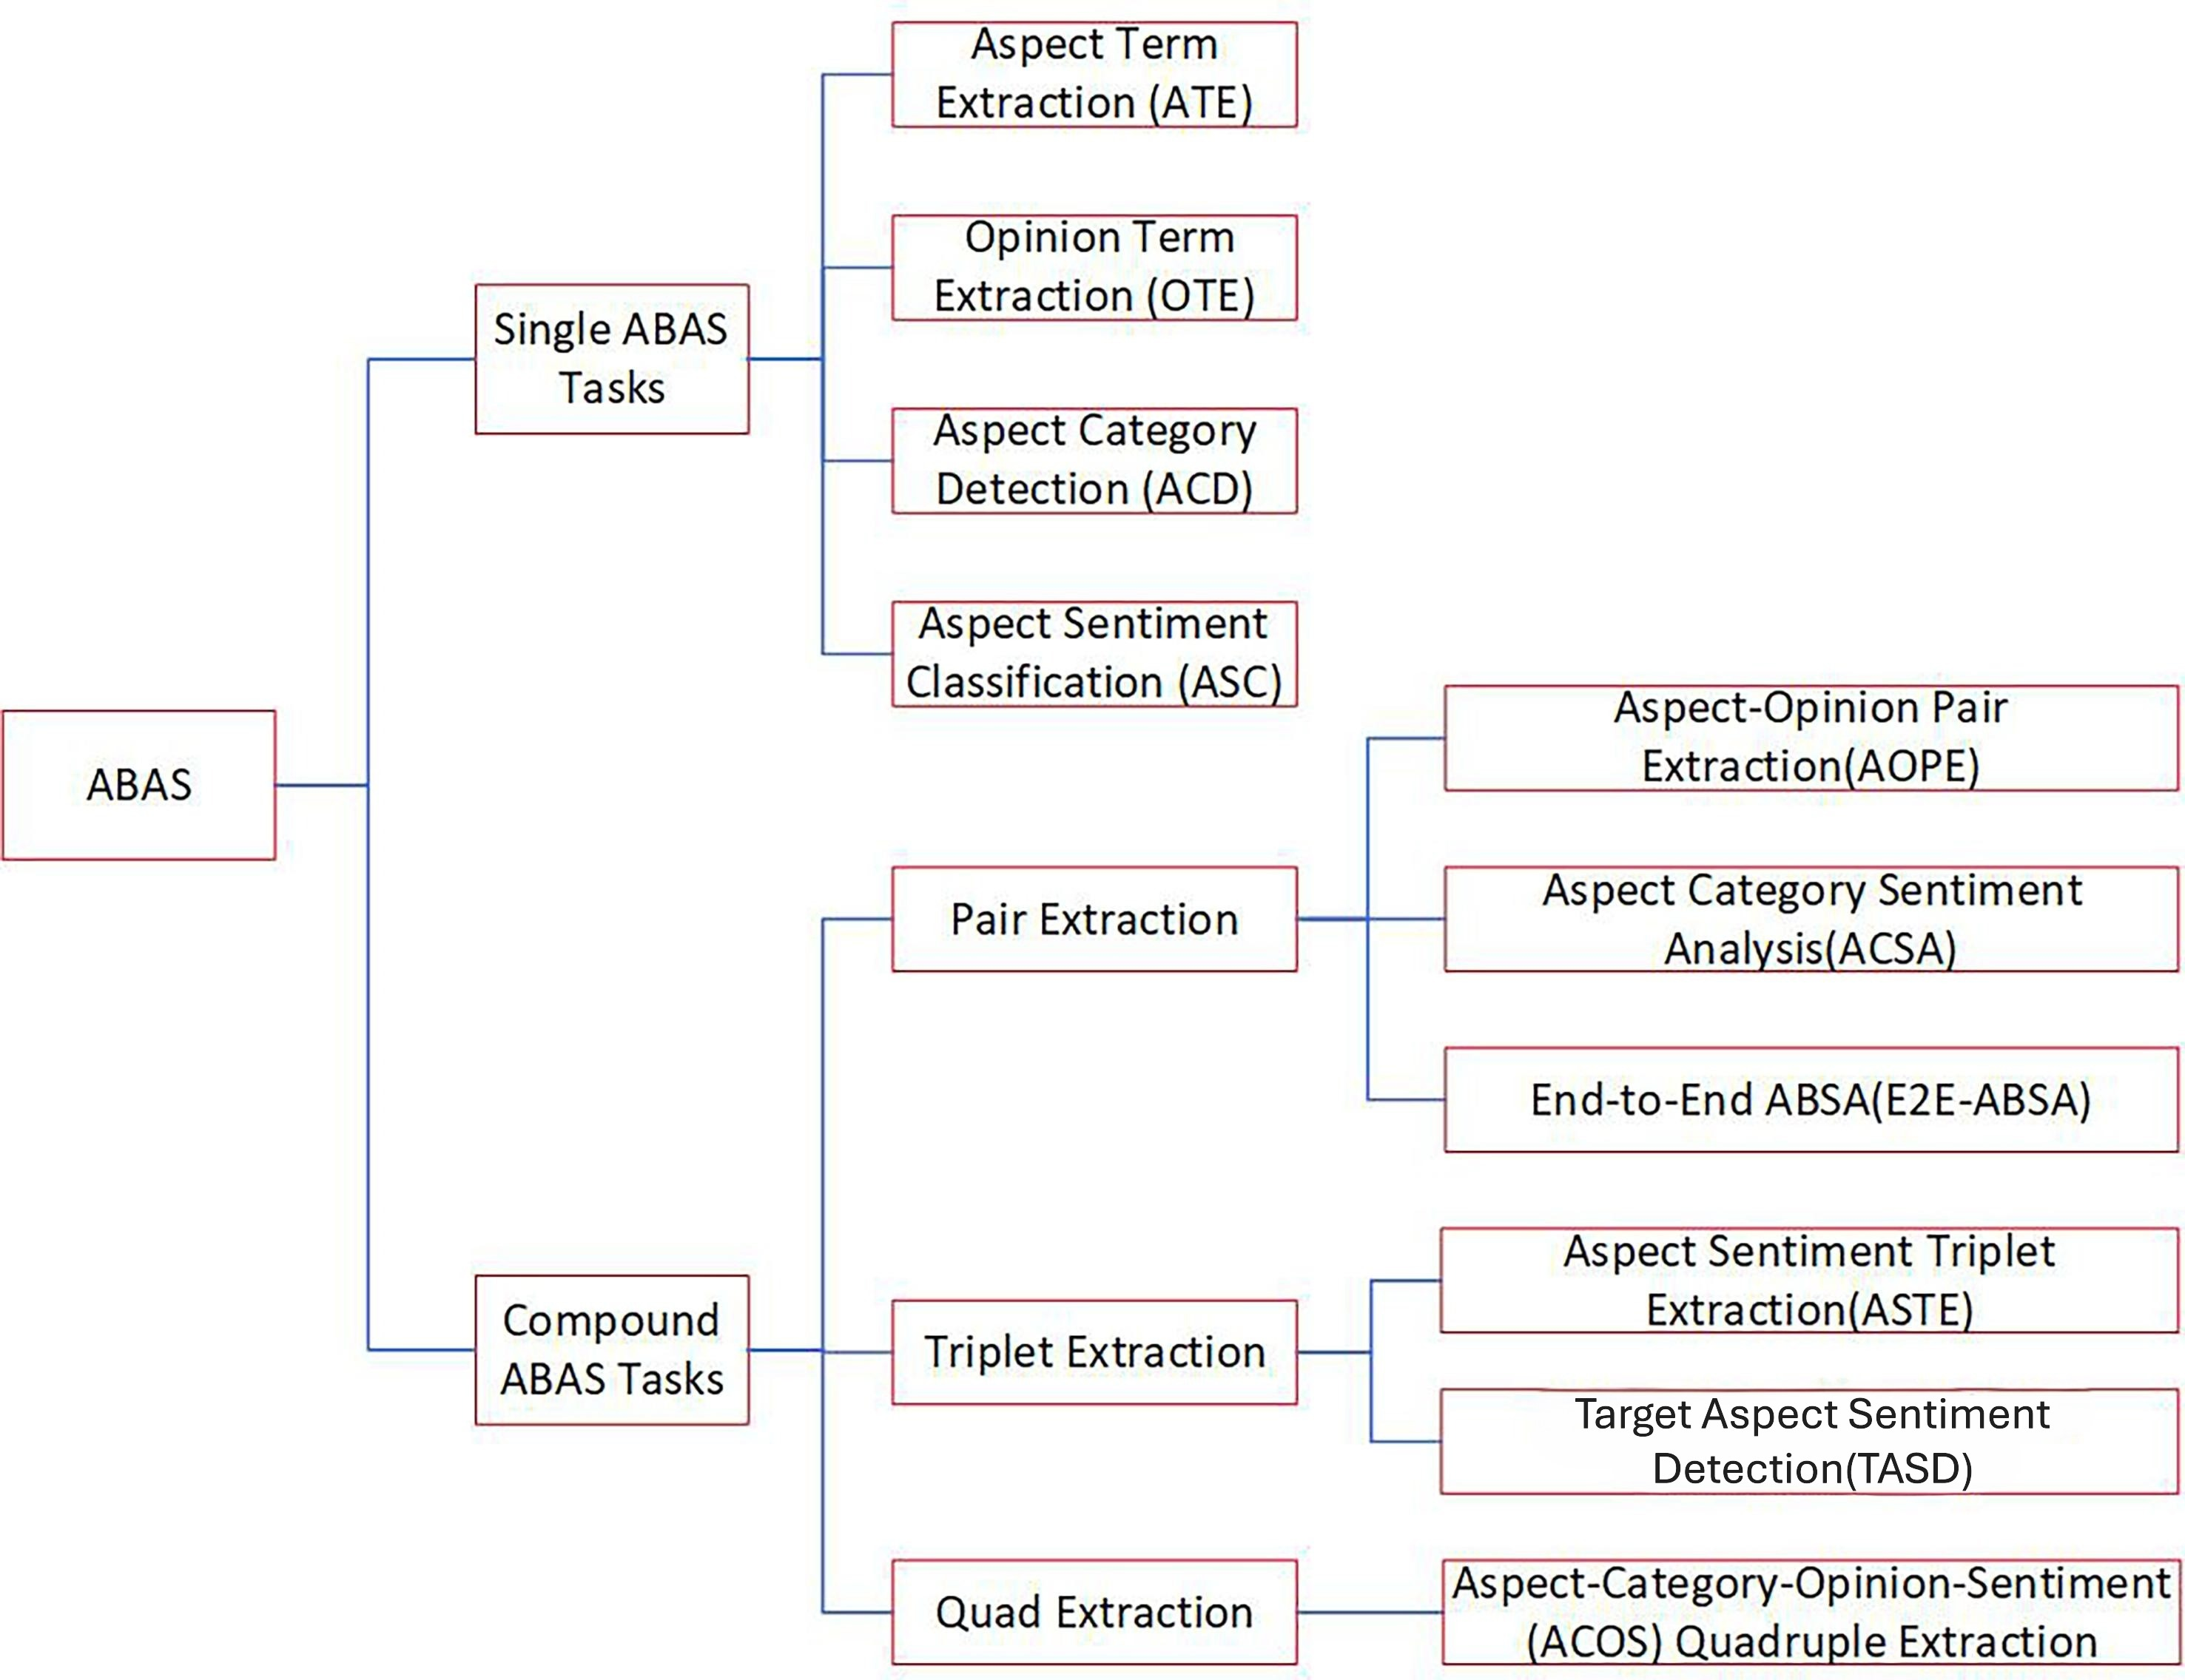
\includegraphics[width=0.9\textwidth]{images/absa}
    \caption[Jednotlivé dílčí úlohy aspektové analýzy sentimentu]%
    {Jednotlivé dílčí úlohy aspektové analýzy sentimentu, upravený obrázek z~\cite{MAO2024102048}}
    \label{fig:ABSA}
\end{figure}
\section{Aspektová analýza sentimentu}\label{absa}
Aspektová analýza sentimentu (ABSA, \emph{Aspect-based sentiment analysis}) je detailní forma analýzy sentimentu, která v poslední době získává významnou pozornost ve výzkumu. Hlavní myšlenkou ABSA je, že emoce nebo názory obsažené v textu se nevztahují pouze na jednu entitu jako celek, ale konkrétně na její určité aspekty či vlastnosti~\cite{TAN2020336}. Výzkum ABSA se obecně zaměřuje na identifikaci sentimentu z několika vzájemně propojených pohledů, zejména na úrovni aspektů, aspektových kategorií, názorových výrazů a polarity sentimentu~\cite{XU2020135}.~\cite{MAO2024102048}

Tato úroveň analýzy sentimentu představuje nejdetailnější stupeň, který lze dále rozčlenit do několika dílčích úloh, zaměřujících se na různé aspekty a jejich vlastnosti. V následujících podsekcích budou nejprve představeny jednotlivé dílčí úlohy aspektové analýzy sentimentu (\emph{Single ABSA Tasks}), a poté budou popsány složitější úlohy (\emph{Compound ABSA Tasks}), vznikající kombinací těchto dílčích úloh, které již poskytují komplexní informace o sentimentu vzhledem k jednotlivým aspektům (viz. Obrázek \ref{fig:ABSA}).

\subsection{Základní dílčí úlohy ABSA}
Aspektová analýza sentimentu zahrnuje čtyři základní dílčí úlohy (tzv. \emph{Single ABSA Tasks}). Konkrétně se jedná o extrakci aspektů (\emph{Aspect Term Extraction, ATE}), extrakci názorových výrazů (\emph{Opinion Term Extraction, OTE}), detekci aspektových kategorií (\emph{Aspect Category Detection, ACD}) a klasifikaci sentimentu aspektů (\emph{Aspect Sentiment Classification, ASC}).~\cite{MAO2024102048}

\begin{itemize}
    \item \textbf{Extrakce aspektů (ATE)} \\
    Cílem této úlohy je identifikace všech aspektů (neboli entit) zmíněných v textu, vůči kterým se následně provádí analýza sentimentu. Jedná se o klíčový krok většiny komplexnějších ABSA úloh, protože definuje hlavní objekty další analýzy.~\cite{zhang2022surveyaspectbasedsentimentanalysis}

    \item \textbf{Extrakce názorových výrazů (OTE)} \\
    Tato úloha spočívá ve vyhledávání slov či frází, které vyjadřují názory nebo postoje, aniž by nutně specifikovaly konkrétní aspekty. Úkolem je tedy získat ze samotného textu výrazy, které se následně přiřazují k relevantním aspektům.~\cite{zhang2022surveyaspectbasedsentimentanalysis}

    \item \textbf{Detekce aspektových kategorií (ACD)} \\
    Tato úloha se věnuje určování obecných kategorií aspektů. Existují zde dva přístupy. První spočívá v kategorizaci aspektů do širších skupin (např. ve větě \uv{Salát byl skvělý, ale náš číšník byl velmi nepříjemný} by výsledkem byly kategorie \uv{jídlo} a \uv{obsluha}~\cite{MAO2024102048}). Druhý přístup využívá kategorie k popisu vlastností jednotlivých aspektů (např. věta \uv{Pokoje jsou skvělé, jsou velmi levné} by vedla ke kategoriím \uv{obecná} a \uv{cena}~\cite{chebolu-etal-2024-oats}).

    \item \textbf{Klasifikace sentimentu aspektů (ASC)} \\
    Tato úloha je přímo zaměřena na určení sentimentu konkrétních aspektů zmíněných v textu. Jde tedy o samotnou analýzu sentimentu, kdy cílem je přiřadit specifikovaným aspektům správnou polaritu sentimentu (pozitivní, negativní či neutrální). Právě tato úloha představuje hlavní zaměření této bakalářské práce.~\cite{zhang2022surveyaspectbasedsentimentanalysis}
\end{itemize}

\subsection{Složené úlohy ABSA}
Jak již bylo zmíněno, složené úlohy ABSA (tzv. \emph{Compound ABSA Tasks}) spojují několik dílčích úloh dohromady, aby bylo možné lépe zachytit a popsat sentiment obsažený v textech. Hlavním cílem těchto úloh je extrahovat a predikovat více sentimentových prvků současně. Mezi typy složených úloh patří extrakce dvojic, trojic a čtveřic sentimentových prvků.~\cite{MAO2024102048}. Jelikož jsou tyto úlohy již nad rámec této práce, budou popsány pouze stručně, podrobnější popis je dostupný v citacích u jednotlivých úloh.

\subsubsection{Extrakce dvojic}
Mezi úlohy založené na extrakci dvojic patří extrakce aspekt-názor dvojic (\emph{Aspect-Opinion Pair Extraction, AOPE}), analýza sentimentu aspektových kategorií (\emph{Aspect Category Sentiment Analysis, ACSA}) a end-to-end aspektová analýza sentimentu (\emph{End-to-End ABSA, E2E-ABSA})~\cite{MAO2024102048}, někdy označovaná jako jednotná aspektová analýza sentimentu (\emph{Unified ABSA, UABSA})~\cite{zhang-etal-2021-towards-generative}. Tyto úlohy poskytují ucelenější pohled na sentiment tím, že spojují jednotlivé prvky analýzy (např. aspekt a odpovídající názor) nebo zároveň určují sentiment vůči daným aspektům.

\begin{itemize}
    \item \textbf{Extrakce aspekt-názor dvojic (AOPE)} \\
    Tato úloha spočívá v extrakci párů tvořených aspektem a k němu náležícím názorovým výrazem. Cílem je identifikovat vazbu mezi konkrétními aspekty a slovy, která je popisují. Například z věty: \uv{Salát byl skvělý a číšník byl také velmi nápomocný} se získají dvojice: \uv{[salát, skvělý]} a \uv{[číšník, nápomocný]}.~\cite{zhang-etal-2021-towards-generative}

    \item \textbf{Analýza sentimentu aspektových kategorií (ACSA)} \\
    Při této úloze se analyzuje sentiment v rámci předem definovaných aspektových kategorií, a tím se určuje celková polarita dané kategorie. Například z věty: \uv{Pití bylo skvělé a jídlo bylo velmi chutné} by se získaly dvojice: \uv{[občerstvení, pozitivní]} a \uv{[občerstvení, pozitivní]}, což dohromady vypovídá o pozitivním sentimentu pro kategorii \uv{občerstvení}.~\cite{li2020multiinstancemultilabellearningnetworks}

    \item \textbf{End-to-End aspektová analýza sentimentu (E2E-ABSA)} \\
    Tato úloha v jednom kroku spojuje extrakci aspektových termínů a jejich klasifikaci sentimentu, tedy zároveň identifikuje aspekty i jejich náladu (polaritu). Například z věty: \uv{Salát byl skvělý a číšník byl také velmi nápomocný} se získají dvojice: \uv{[salát, pozitivní]} a \uv{[číšník, pozitivní]}.~\cite{zhang-etal-2021-towards-generative}
\end{itemize}

\subsubsection{Extrakce trojic}
Mezi úlohy založené na extrakci trojic patří extrakce aspekt-názor-sentiment trojic (\emph{Aspect Sentiment Triplet Extraction, ASTE}) a detekce aspekt-kategorie-sentiment (\emph{Target Aspect Sentiment Detection, TASD}).~\cite{MAO2024102048} Tyto úlohy přinášejí podrobnější popis sentimentu tím, že identifikují nejen aspekty, ale i jejich názory či vlastnosti a sentiment současně.

\begin{itemize}
    \item \textbf{Extrakce aspekt-názor-sentiment trojic (ASTE)} \\
    Cílem této úlohy je identifikovat trojici tvořenou aspektem, k němu příslušným názorovým výrazem a polaritou sentimentu. Poskytuje detailní a přesný vhled do hodnocení, protože zohledňuje, \emph{co} je hodnoceno (aspekt), \emph{jaký} je k němu sentiment a případně \emph{proč} (na základě čeho). Například z věty: \uv{Salát byl skvělý a číšník byl také velmi nápomocný} lze získat trojice: \uv{[salát, skvělý, pozitivní]} a \uv{[číšník, nápomocný, pozitivní]}.~\cite{MAO2024102048, Peng_Xu_Bing_Huang_Lu_Si_2020}

    \item \textbf{Cílená aspektová analýza sentimentu (TASD)} \\
    Tato úloha spočívá v detekci kategorií aspektů, konkrétních aspektů a jejich sentimentové polarity. Hlavním cílem je určit, do jaké kategorie daný aspekt spadá a jakou má polaritu. Například z věty \uv{I přesto, že pizza byla vážně skvělá, cena byla velmi vysoká} lze odvodit trojice: \uv{[pizza, jídlo\#kvalita, pozitivní]} a \uv{[pizza, jídlo\#cena, negativní]}, čímž se vyjádří, že pizza je sice kvalitní, avšak poměrně drahá.~\cite{Wan_Yang_Du_Liu_Qi_Pan_2020, Ke2023}
\end{itemize}

\subsubsection{Extrakce čtveřic}
Nejkomplexnější úlohou v ABSA je extrakce čtveřic, konkrétně jde o extrakci čtveřic aspekt-kategorie-názor-sentiment (\emph{Aspect-Category-Opinion-Sentiment Quadruple Extraction, ACOS})~\cite{MAO2024102048}. Tato úloha integruje všechny základní prvky aspektové analýzy sentimentu a umožňuje nejdetailnější pohled na postoje vyjádřené v textu.

\begin{itemize}
    \item \textbf{Extrakce čtveřic aspekt-kategorie-názor-sentiment (ACOS)} \\
    Tato úloha představuje nejkomplexnější formu extrakce, při které se získávají kompletní čtveřice obsahující konkrétní aspekt, jeho kategorii, odpovídající názor a sentiment. Jako příklad lze uvést větu: \uv{Vypadá pěkně a jeho konstrukce je velice bytelná.} Z této věty je možné získat čtveřice: \uv{[povrch, design, bytelná, pozitivní]} a \uv{[null, design, pěkně, pozitivní]}. V některých případech nemusí být všechny složky čtveřice ve větě explicitně vyjádřeny, což představuje další výzvu této úlohy.~\cite{MAO2024102048, cai-etal-2021-aspect}
\end{itemize}

\subsection{Využití transformátorových modelů v ABSA}
V sekci \ref{TechAnaSen} byly představeny různé metody analýzy sentimentu. Stále více studií se však v současné době zaměřuje na využití transformátorové architektury~\cite{vaswani2023attentionneed}, například modelu BERT~\cite{devlin2019bert} a jeho odvozených variant. Tato část proto popisuje práce, které aplikují BERT na jednotlivé metody ABSA, srovnávají jej s dalšími modely a zkoumají jeho vhodnost v různých doménách i jazycích. Také v této práci budou použity vybrané varianty modelů BERT, a to jak pro různé jazyky, tak pro různé okruhy dat.

\subsubsection{Datasety}
Kvalitní a dostatečně rozsáhlá trénovací data představují klíčový předpoklad úspěchu při trénování modelů. V kontextu analýzy sentimentu, a především u složitějších úloh ABSA, ovšem není dostupných datasetů mnoho. Proto některé studie usilují o tvorbu nových datových sad, jež obsahují větší množství domén, více sentimentů v jedné větě či rozsáhlejší objem dat. Na těchto nových korpusech následně testují výkonnost modelů typu BERT, aby ověřily jejich schopnost zachytit jemné nuance aspektové analýzy.

\begin{itemize}
    \item \textbf{Dataset OATS} \\
    V datové sadě OATS (\emph{Opinion Aspect Target Sentiment})~\cite{chebolu-etal-2024-oats} je cílem připravit objemnější datasety a rozšířit dosavadní spektrum domén (často omezené na recenze notebooků nebo restaurací~\cite{pontiki-etal-2014-semeval}) o další oblasti, jako jsou potraviny (Amazon Food Reviews), online kurzy (Coursera) a hotely (TripAdvisor). Tento dataset je připraven pro několik složených ABSA úloh (E2E-ABSA, ASTE, TASD a ACOS).

    \item \textbf{Dataset MAMS} \\
    Cílem datové sady MAMS (\emph{Multi-Aspect Multi-Sentiment})~\cite{jiang-etal-2019-challenge} je zajistit, aby každá věta obsahovala alespoň dva hodnocené aspekty. Data pocházejí z kolekce CitySearch New York a jsou uzpůsobena primárně pro úlohy E2E-ABSA a ACSA.
\end{itemize}

\subsubsection{Složené úlohy ABSA}
Pro jednotlivé složené úlohy ABSA existuje řada studií, které se zaměřují na hlubší pochopení daných problémů či na formulaci nových variant těchto úloh. V této sekci jsou stručně představeny vybrané práce, jež nabízejí nové pohledy a přístupy.

\begin{itemize}
    \item \textbf{ACSA}
    \begin{itemize}
        \item Jednou z hlavních výzev ACSA je skutečnost, že k jedné kategorii se v jedné větě může vztahovat více názorů. Tento problém řeší například autoři studie~\cite{li2020multiinstancemultilabellearningnetworks}, kteří nejprve vyhledají v textu konkrétní instance aspektových kategorií, přiřadí jim sentiment a následně určí výslednou polaritu pro danou kategorii. 
        
        \item V práci~\cite{LIU2023110339} autoři navrhují model KASA, který tuto úlohu pojímá jako klasifikaci dvojice vět (sentence-pair classification) namísto klasifikace jedné věty (single-sentence classification), čímž ji činí jednodušší k řešení.
    \end{itemize}

    \item \textbf{E2E-ABSA}
    \begin{itemize}
        \item V~\cite{li-etal-2019-exploiting} je popsáno využití modelu BERT a jeho upravených verzí pro End-to-End ABSA. Ve srovnání se staršími modely (např. LSTM) dosahoval BERT výrazně lepších výsledků. Navíc autoři sjednocují porovnání modelů tím, že důsledně využívají samostatný (hold-out) vývojový dataset pro ladění modelu, což dřívější studie často přehlížely. Díky tomu jejich řešení slouží jako BERT-based benchmark pro E2E-ABSA.
    
        \item Autoři studie~\cite{toledo-ronen-etal-2022-multi} se naopak soustředí na vývoj takového modelu pro analýzu sentimentu, který lépe obstojí v různých doménách, a snaží se tak vyřešit problém omezení modelů na konkrétní doménu, jež vyplývá z použití doménově specifických datasetů pro fine-tuning.
    \end{itemize}

    \item \textbf{ASTE}
    \begin{itemize}
        \item Práce~\cite{zhang-etal-2022-boundary} převádí reprezentaci trojic do \uv{relační oblasti} (relation region) v 2D tabulce a pojímá úlohu ASTE jako detekci a klasifikaci těchto oblastí.
        \item Ve studii~\cite{mukherjee-etal-2021-paste} je představen \uv{přístup bez značkování} (tagging-free), který lépe zachycuje vzájemnou závislost mezi komponentami trojice. Autoři využívají architekturu typu encoder-decoder v kombinaci s modelem BERT.
    \end{itemize}

    \item \textbf{TASD}
    \begin{itemize}
        \item Ve studii~\cite{wu2020contextguidedberttargetedaspectbased} autoři rozšiřují BERT o dodatečný kontext a sledují dopady této úpravy na výkonnost modelu. Zároveň poukazují na to, že rozšíření předtrénovaných modelů typu self-attention o kontextové závislosti dokáže významně zlepšit výsledky v kontextově orientovaných jazykových úlohách.
        \item V~\cite{sun-etal-2019-utilizing} se ověřuje, nakolik se zlepší přesnost predikce, pokud je \emph{TASD} pojato jako klasifikace dvojice vět (sentence-pair classification), například formou otázky a odpovědi. Tento přístup je použit i v této práci, kde bude porovnán s klasifikací jedné věty (single-sentence classification).
        \item Někdy aspekt (target) není ve větě explicitně zmíněn, nýbrž pouze naznačen. Příklad: \uv{Jídlo přišlo po 20 minutách a bylo studené.} -- je zde explicitní trojice s aspektem \uv{jídlo}, avšak lze rovněž odvodit negativní hodnocení \uv{obsluhy}, neboť jídlo dorazilo pozdě. Tím se zabývá studie~\cite{Wan_Yang_Du_Liu_Qi_Pan_2020}.
        \item V~\cite{Ke2023} se výzkumníci snaží řešit \emph{TASD} prostřednictvím \uv{systému využívajícího prompty} (prompt-based system), kde je generována otázka a k ní odpověď. Autoři rovněž navrhují vlastní řešení, jak tento přístup aplikovat v praxi.
    \end{itemize}

    \item \textbf{ACOS}
    \begin{itemize}
        \item Ve studii~\cite{cai-etal-2021-aspect} autoři popisují tuto komplexní úlohu, která propojuje všechny dílčí ABSA úlohy, a zároveň vytvářejí datasety Restaurant-ACOS a Laptop-ACOS. Své řešení testují na čtyřech různých systémech, jejichž podrobný popis je uveden v originálním díle.
        \item V~\cite{Li2023-wo} je navržena metoda pro extrakci čtveřic, jež zohledňuje vzdálenost mezi aspekty a názorovými výrazy. Autoři následně porovnávají své výsledky na datasetech Restaurant-ACOS a Laptop-ACOS s jinými přístupy, přičemž dosahují lepších výkonnostních ukazatelů.
    \end{itemize}

\end{itemize}

\section{Využití analýzy sentimentu}
Analýza sentimentu nachází uplatnění v celé řadě oblastí. Díky rozmachu internetu a snadné dostupnosti pro uživatele sdílet své názory a pocity se význam tohoto přístupu neustále zvyšuje. Firmy a organizace mohou na základě recenzí a komentářů efektivně upravovat své produkty a služby, a tím zvyšovat zisk. V oblasti zdravotnictví lze analýzu sentimentu využít například ke sledování potenciálních sebevražedných myšlenek prostřednictvím detekce negativních emocí ve veřejně publikovaných příspěvcích.~\cite{kumar2023comprehensivereviewsentimentanalysis} V následujících podsekcích jsou stručně představeny hlavní oblasti, kde se analýza sentimentu uplatňuje, a uvedeny studie, které se danou tématikou zabývají.

\subsection{Obchodní oblast}
Analýza sentimentu představuje v obchodní sféře jeden z nejvýznamnějších nástrojů pro zlepšování produktů a služeb. Díky schopnosti zpracovat velké množství recenzí lze účinně odhalovat nedostatky a identifikovat příležitosti ke zkvalitnění nabídky. Některé studie~\cite{Sreesurya2020, KUMAR201941} podrobně popisují proces extrakce sentimentu a jeho praktické využití v obchodním prostředí. Další práce se zaměřují na analýzu dat získaných z Amazonu~\cite{BoseSentiment}, z čínských online recenzí~\cite{Wang12022016}, z Facebooku~\cite{Baj-Rogowska} či ze služby Zomato~\cite{9574641}. Souhrnně se těmito tématy zabývají také publikace~\cite{kumar2023comprehensivereviewsentimentanalysis, MAO2024102048, BIRJALI2021107134}.

Analýza sentimentu nemusí sloužit pouze velkým firmám a organizacím, ale nabízí také přínos pro jednotlivce zajímající se o finanční trhy, akcie či kryptoměny. Řada studií~\cite{TadleFOMC, DohHowtoSay, Xing2018} se věnuje využití sentimentu při odhadech vývoje cen akcií a zkoumá, zda pozitivní či negativní nálada může signalizovat budoucí růst nebo pokles. Podobně existují i práce zaměřené na kryptoměny~\cite{ROGNONE2020101462, KRAAIJEVELD2020101188}, které zkoumají, do jaké míry lze sentiment využít pro predikci cenového vývoje. Přehledně se tímto tématem zabývají též díla~\cite{kumar2023comprehensivereviewsentimentanalysis, MAO2024102048, BIRJALI2021107134}.

Analýza sentimentu se nemusí zaměřovat pouze na recenze produktů a služeb, ale lze ji využít i k mapování obecných postojů k aktuálním událostem. Řada studií~\cite{ManguriCovid, NaseemCovid, CHAKRABORTY2020106754, ALAMOODI2021114155, Abd-Alrazaq} například zkoumá reakce uživatelů sociálních sítí (zejména X, původně Twitter) na pandemii COVID-19. Další výzkumy se věnují jiným tématům, jako je rusko-ukrajinská válka~\cite{baker2023prediction} či postoje k elektromobilům v kontextu rostoucích cen pohonných hmot~\cite{JihadEV}. Přehledný souhrn těchto výzkumů nabízejí také články~\cite{kumar2023comprehensivereviewsentimentanalysis, MAO2024102048}.

\subsection{Doporučující systémy}
Analýza sentimentu nachází uplatnění i v doporučujících systémech, ať už jde o hotely či filmy. Typickým přístupem je práce s recenzemi konkrétního uživatele, na jejichž základě lze určit, co by mu mohlo být doporučeno. Různé metody a postupy pro návrh doporučujících systémů popisují studie~\cite{SHEN2019249, LI2016164, SERRANOGUERRERO2020106768, RAY2021106935, FU2020106803}, jejichž souhrn je uveden v~\cite{BIRJALI2021107134}.

\subsection{Zdravotnická oblast}
V předchozích oblastech byla analýza sentimentu popsána především ve vztahu k ekonomickým přínosům, ať už pro firmy nebo pro jednotlivce. Tato metoda však nachází uplatnění i při zlepšování zdravotního stavu populace. Lze ji například využít ke sledování názorů veřejnosti na lékaře, léčiva a zdravotní péči~\cite{JIMENEZZAFRA201950, Ramírez-Tinoco2019, clark2018sentimentanalysisbreastcancer}, nebo k monitorování ohrožených skupin, jako jsou senioři~\cite{Ayata2020}, případně k detekci sebevražedných myšlenek a depresí na základě příspěvků na sociálních sítích~\cite{Desmet2013, Wang2013, Jung2017}. Dokonce existují studie, které se zaměřují na predikci výskytu rakoviny tlustého střeva a konečníku~\cite{Baker2023}. Podrobnější popis uvedených aplikací nabízí např. díla~\cite{kumar2023comprehensivereviewsentimentanalysis, MAO2024102048, BIRJALI2021107134}.

Analýza sentimentu se přitom nemusí týkat pouze fyzického zdraví. Lze ji použít i pro prevenci vulgárních či nenávistných projevů na internetu a tím bránit psychické zdravý online uživatelů. Negativní a urážlivé výrazy mohou u uživatelů vyvolávat stres nebo přispívat k rozvoji depresí. Řada studií se proto zabývá detekcí nenávistných projevů (hate speech) například na X (Twitter)~\cite{Jiang2019, Badjatiya_2017}, Facebooku~\cite{8669073} či analýzou kyberšikany na Instagramu~\cite{Zidny2019}. Souhrnné informace o těchto využitích lze nalézt v~\cite{kumar2023comprehensivereviewsentimentanalysis}.

\section{Otevřené problémy analýzy sentimentu}
Ačkoli se koncept analýzy sentimentu může na první pohled zdát jednoduchý (určitý názor je buď pozitivní, negativní či neutrální), v praxi se často objevují situace, kdy tatáž slova mohou v různém kontextu nést kladný i záporný význam. Člověk tyto nuance rozeznává intuitivně, avšak pro počítačové zpracování představují značnou výzvu. Následující paragrafy nastíní některé z hlavních problémů a otevřených otázek v oblasti analýzy sentimentu. Podrobnější rozbor a další problémy lze nalézt v~\cite{kumar2023comprehensivereviewsentimentanalysis, MAO2024102048, BIRJALI2021107134}.

\paragraph{Sarkasmus}
Sarkasmus se v běžném životě vyskytuje poměrně často, někteří lidé ho používají prakticky denně. Pro klasickou analýzu textu však představuje problém, protože věta, která vypadá na první pohled pozitivně, může být ve skutečnosti míněna ironicky. Různé studie uvedené v~\cite{BIRJALI2021107134} se proto zaměřují na rozpoznávání a správnou interpretaci sarkasmu.

\paragraph{Vícejazyčná analýza sentimentu}
Většina současných výzkumů se soustředí převážně na angličtinu, jelikož pro ni existuje relativně velké množství dat a dalších jazykových zdrojů. U jazyků s nedostatečnou podporou (tzv. \emph{low-resource languages}) je však problematické získat dostatečné datasety pro předtrénování modelů, natož pro samotnou analýzu sentimentu~\cite{BIRJALI2021107134}. Komplikací bývají i texty, v nichž se mísí více jazyků (tzv. \emph{code-switching}), jelikož pro tuto oblast dosud chybějí rozsáhlejší zdroje dat. Podrobnější rozbor těchto obtíží je k dispozici v~\cite{kumar2023comprehensivereviewsentimentanalysis, MAO2024102048, BIRJALI2021107134}.

\paragraph{Problém domén}
Datasety pro trénování analýzy sentimentu obvykle pocházejí pouze z jedné oblasti, například z recenzí notebooků či restaurací~\cite{pontiki-etal-2014-semeval}. Modely se tak naučí rozpoznávat sentiment především v dané doméně, což je nevýhodou při nasazení do jiného kontextu. Některé výrazy, které mají v recenzích notebooků pozitivní význam, se totiž v jiných oblastech nemusí projevovat stejně.~\cite{kumar2023comprehensivereviewsentimentanalysis, MAO2024102048, BIRJALI2021107134}
